\setcounter{chapter}{18}
\chapter{Teste 1 2019/20}
\section{Pergunta 1}
{
\renewcommand{\thesubsection}{\thesection\alph{subsection}}
\begin{equation*}
	e^x-x-2-9=0 \iff e^x-x-11=0
\end{equation*}
\subsection{Item a}
\lstinputlisting[language=Maxima, caption=Maxima input 2019T1-1a]{2019T1_1a.mc}
\begin{center} 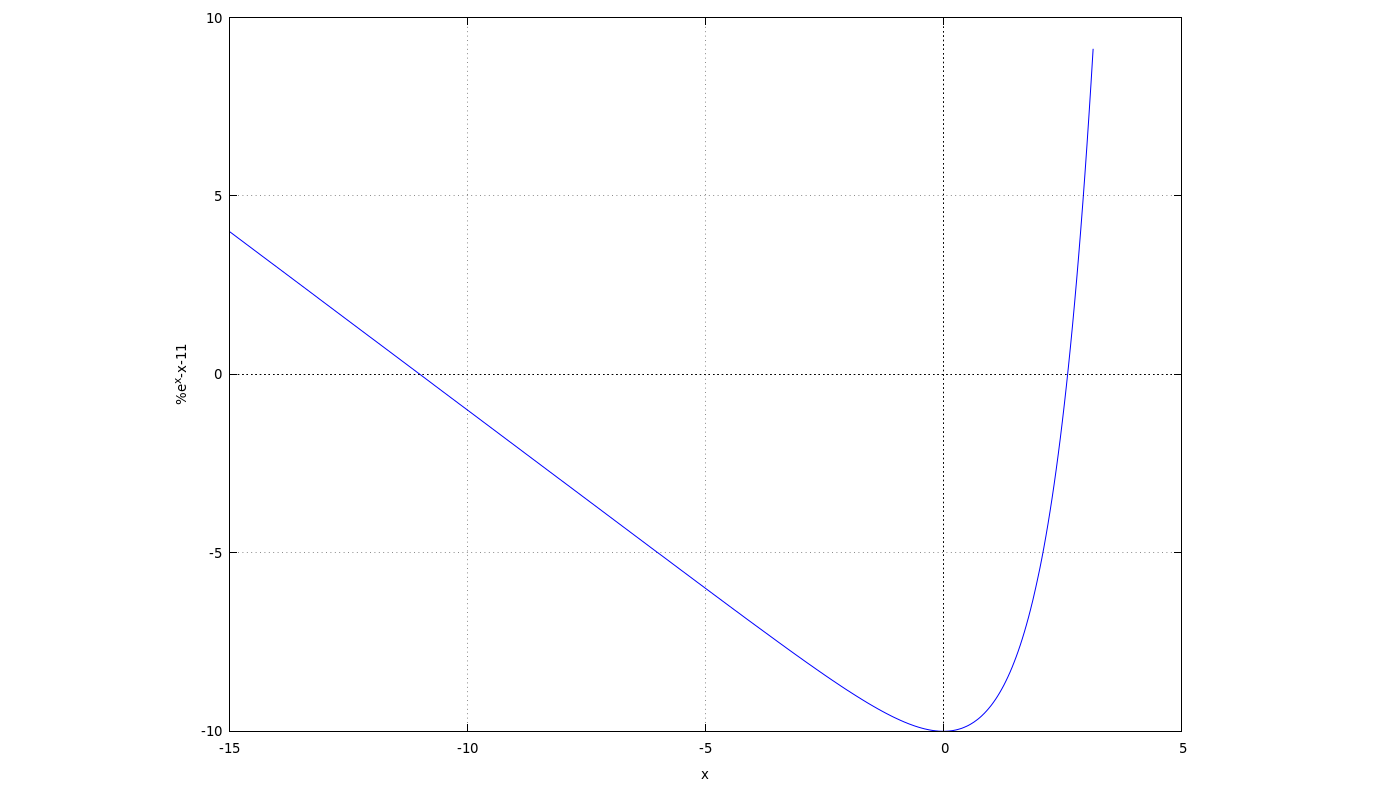
\includegraphics[scale=0.32]{2019T1_1a} \end{center}
A visualização do gráfico da função permite verificar que existem duas raízes:
\begin{itemize}
	\item $x_1 \in [-12,-10]$, a função passa de positiva $f(-12)=1.000006$ para negativa $f(-10)=-0.999954$. $x_1 = -10.999983$
	\item $x_2 \in [2,3]$ a função passa de negativa $f(2)=- 5.610944$ para positiva $f(3)=6.085537$. $x_2=2.610869$
\end{itemize}

\subsection{Item b}
\begin{alignat*}{2}
f(x)=e^x-x-11 \iff f'(x)=e^x-1
\end{alignat*}
\begin{alignat*}{2}
g_0(x)
&=x-\frac{f(x)}{f'(x)} \\
&=x-\frac{e^x-x-11}{e^x-1}\\
&=x+\frac{-e^x+x+11}{e^x-1}\\
&=\frac{xe^x-x-e^x+x+11}{e^x-1}\\
&=\frac{e^x(x-1)+11}{e^x-1}
\end{alignat*}
\begin{alignat*}{2}
x_{n+1}
&=g_0(x_n) \\
&=\frac{e^{x_n}(x_n-1)+11}{e^{x_n}-1}
\end{alignat*}
\subsection{Item c}
\lstinputlisting[language=Maxima, caption=Maxima input 2019T1-1c]{2019T1_1c.mc}

Pelo critério $|g_0'(x)|<1$, a fórmula 0 converge em aprox. $(-\infty,-2.33)$ e em aprox. $(2.00,+\infty)$.\\
Através de uma análise exploratória, pude concluir que, para guess $x_0$, a fórmula 0:
\begin{itemize}
	\setlength{\itemindent}{-1.5em}
	\item Em $\in (-\infty,0)$ converge para $x_1$ 
	\item Em $\in (0,+\infty)$ converge para $x_2$
	\item Em $x_0=0$ ocorre divisão por $0$ na 1ª iteração
\end{itemize}
\begin{center} 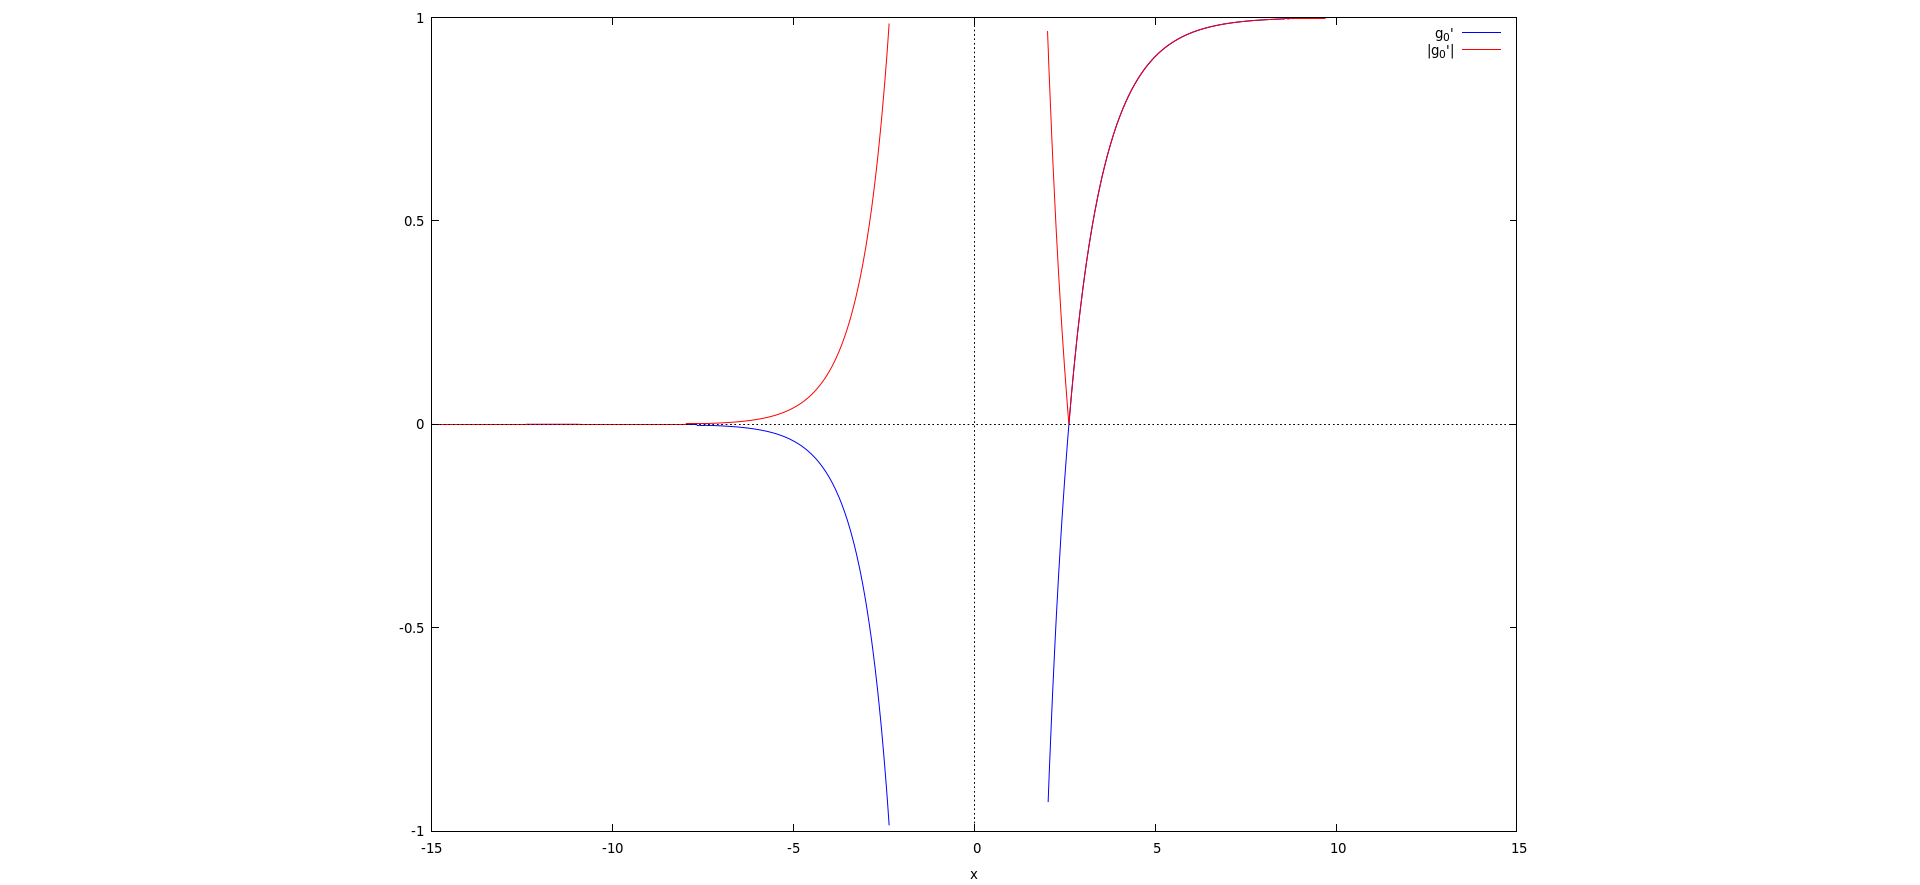
\includegraphics[scale=0.2,trim={14cm 0 14cm 0},clip]{2019T1_1c0} \end{center}
Pelo critério $|g_1'(x)|<1$, a fórmula 1 converge em $(-\infty,0)$.\\
Através de uma análise exploratória, pude concluir que, para guess $x_0$, a fórmula 1:
\begin{itemize}
	\item Em $(-\infty,x_2)$ converge para $x_1$
	\item Em $x_0=x_2$ devolve sempre $x_2$
	\item Em $(x_2,+\infty)$ diverge
\end{itemize}
\begin{center} 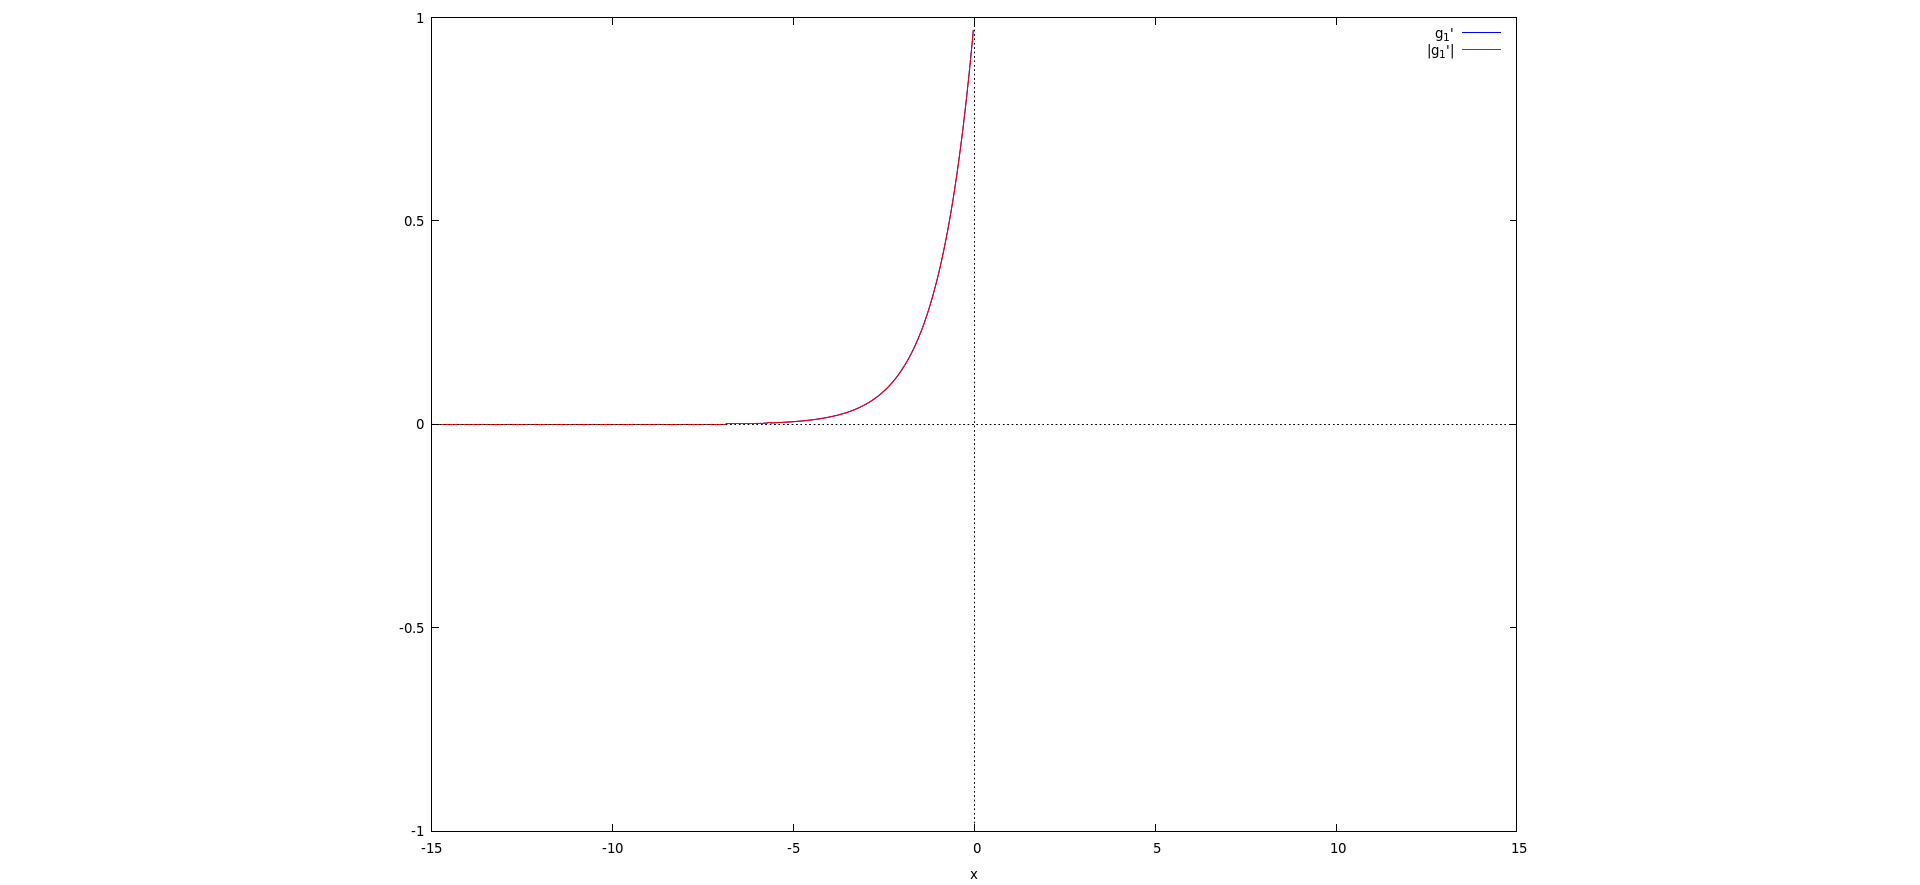
\includegraphics[scale=0.2,trim={14cm 0 14cm 0},clip]{2019T1_1c1} \end{center}

A fórmula $g_2$ apenas possui domínio em $(-11,+\infty)$, por isso podemos ignorar a parte do gráfico em que $x \in (-\infty, -11]$.\\
Pelo critério $|g_2'(x)|<1$, a fórmula 2 converge em aprox. $(-10.01, +\infty)$.\\
Através de uma análise exploratória, pude concluir que, para guess $x_0$, a fórmula 2:
\begin{itemize}
	\item Em $(-\infty, -11)$ ocorre erro de domínio na 1ª iteração
	\item Em $[-11,x_1)$ ocorre erro de domínio na 2ª ou maior iteração
	\item Em $x_0=x_1$ devolve sempre $x_1$
	\item Em $(x_1,+\infty)$ converge para $x_2$
\end{itemize}
\begin{center} 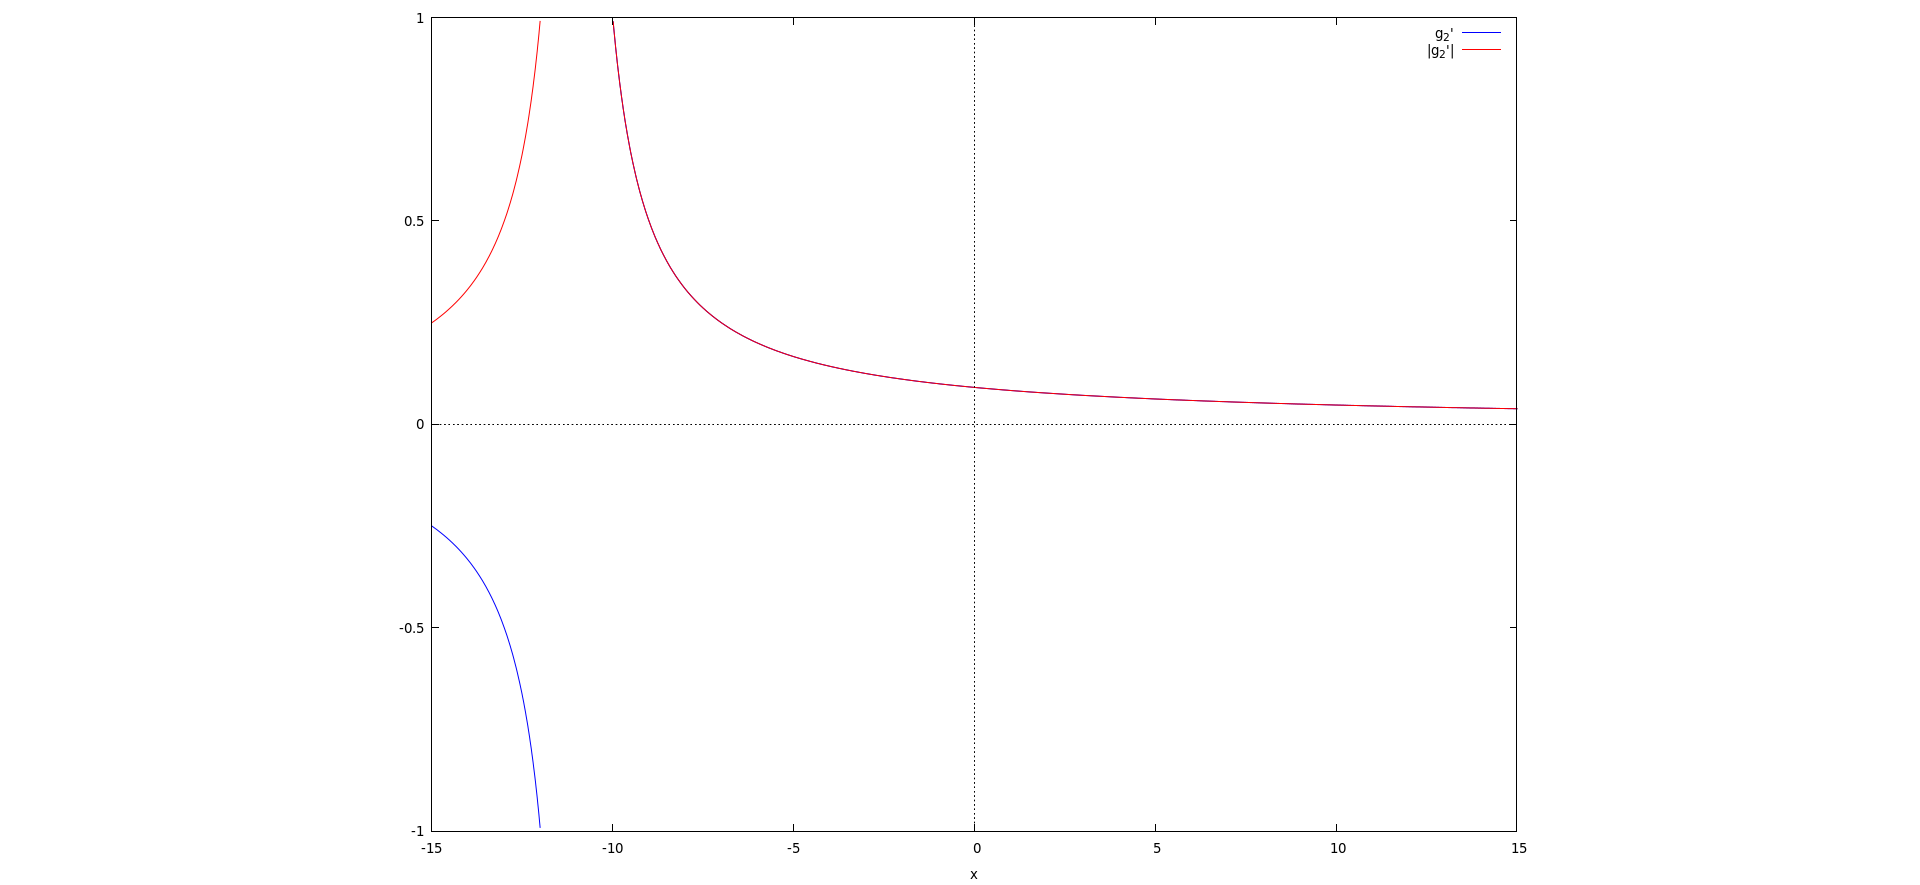
\includegraphics[scale=0.2,trim={14cm 0 14cm 0},clip]{2019T1_1c2} \end{center}
A análise exploratória foi realizada de forma mais fina através da aplicação das fórmulas algumas vezes com Maxima, e de forma mais abrangente com o seguinte programa:
\lstinputlisting[language=Python, caption=Programa 2019T1-1c (Python3)]{2019T1_1c.py}
\subsection{Item d}
Pela alínea anterior, a fórmula 1 só "converge" para $x_2$ quando o guess é exatamente $x_2$, o que se revela inútil porque significa que (1) já teríamos que saber o valor de $x_2$ à partida, ou (2) fazer alguns testes de estabilidade para encontrar o valor de $x_2$, uma vez que, na vizinhança de $x_2$, valores menores que $x_2$ divergem de $x_2$ para baixo e valores maiores que $x_2$ divergem de $x_2$ para cima.
\lstinputlisting[language=Python, caption=Programa 2019T1-1d (Python3)]{2019T1_1d.py}
Utilizando as fórmulas 0 e 2, é devolvido aproximadamente o mesmo valor:
\begin{equation*}
	x_2 = 2.610868638149876
\end{equation*}
A velocidade de convergência depende da capacidade da fórmula de recorrência afetar de forma mais significativa o resultado em função do seu argumento na respetiva região de convergência, e a capacidade de afetar o resultado está ligado ao valor absoluto da derivada da fórmula utilizada.
Utilizando sempre como critério de paragem um valor de erro relativo menor que $10^{-12}$ entre iterações consecutivas, a paragem pela fórmula 1 a partir do guess $x=20$ ocorreu depois de 23 iterações, enquanto que pela fórmula 2 ocorreu depois de 13 iterações. Isto explica-se pelo facto de $|g_0'(x)|$ possuir um valor geralmente próximo de, e inferior a, $1$ na região de convergência a que o guess $x=20$ pertence, enquanto que $|g_2'(x)|$ é menor nessa região de covergência (inferior a 0.1), pelo que a fórmula 0 converge mais rapidamente para o resultado pretendido quando o guess inicial se encontra relativamente longe do resultado final.\\
No entanto, se o valor inicial for mais próximo do valor real, como por exemplo $x=2.61$, a convergência pela fórmula 0 ocorre em 3 iterações, enquanto que pela fórmula 2 ocorre em 9 iterações. Isto explica-se pelo facto de que $|g_0'(x)|$ diminui na vizinhança de $x_2$ até chegar a $0$, enquanto que $|g_2'(x)|$ possui um valor "significativamente" maior do que $0$ (pelo menos 0.06) que permite uma convergência rápida na vizinhança de $x_2$.\\
Em suma:
\begin{itemize}
	\item $g_1$: não converge de forma útil para $x_2$
	\item Desempenho: $g_0$ melhor para guesses longe de $x_2$, $g_2$ melhor na vizinhança de $x_2$
	\item Domínio: $g_2$ converge para $x_2$ em $(x_1,+\infty)$ e $g_0$ em $(0,+\infty)$. No entanto é perigoso usar $g_2$ na proximidade de $0$, uma vez que um valor próximo de $0$ na 1ª iteração tem como resultado um valor muito grande, que quando fornecido na 2ª iteração pode facilmente provocar overflow dado que $g_2$ possui uma exponencial de $x$.
\end{itemize}
\section{Pergunta 2}
\begin{center} \begin{tabular}{r | l}
	\textbf{Item} & \textbf{Resposta} \\ \hline
	(a) & Bisseção \\
	(b) & Bisseção \\
	(c) & Bisseção \\
	(d) & Picard-Peano
\end{tabular} \end{center}
\section{Pergunta 3}
\lstinputlisting[language=Maxima, caption=Maxima input 2019T1-3]{2019T1_3.mc}
\begin{center} \begin{tabular}{c | c c c}
	& Iter. 0 & Iter. 1 & Iter. 2\\ \hline
	$x_n$ & -1.00000 & -1.2291129 & -1.0104435 \\
	$y_n$ & 0.50000 & 1.2744971 & 1.1226234
\end{tabular} \end{center}
\section{Pergunta 4}
O método da falsa posição é um método intervalar, que consiste em, tendo um intervalo $[a,b]$ a que a raiz pertence, traçar uma corda entre os pontos $(a, f(a))$ e $(b, f(b))$, e utilizar o valor $c$ em que a corda interseta o eixo das abcissas como novo limite do intervalo (se $f(c) < 0$, $b$ passa a ser $c$, caso contrário $a$ passa a ser $b$).\\
Na forma normal do método, a garantia de convergência nos dois limites intervalares só existe se o sentido da concavidade da função mudar na raiz, caso contrário o método converge em apenas um dos limites intervalares.\\
Para ultrapassar esta situação, pode-se implementar uma melhoria deste método que consiste em utilizar metade do valor da função no ponto que não foi atualizado na iteração anterior.\\
Outra alternativa seria, em vez de usar como critério de paragem a largura do intervalo, usar um critério de paragem semelhante aos métodos não-intervalares de avaliação da diferença entre estimativas consecutivas. Neste caso, seriam avaliadas as estimativas consecutivas na extremidade do intervalo que está a convergir. Desta forma não é necessário desistir completamente do método da falsa posição.
}